% !TEX root = tracking.tex
\section{Offline Computation \label{sec:precomp}}
The offline computation begins with setting up a pursuit-evasion game \cite{Huang11, Chen17} between the tracking system and the planning system, which we then analyze using HJ reachability. In this game, the tracking system is the pursuer, and the planning system is the evader. In reality the planner is typically not actively trying to avoid the tracking system, but this allows us to account for worst-case scenarios. Assuming both systems act optimally, we want to determine the largest relative distance that may occur over time. This distance is the maximum possible tracking error ($\TEB$).

\subsection{Relative Dynamics}
To determine the relative distance that may occur over time, we first define relative states and dynamics between the tracking and planning models. The individual dynamics are defined in (\ref{eq:tdyn}) and (\ref{eq:pdyn}). The relative system is found by fixing the planning model to the origin and finding the dynamics of the tracking model relative to the planning model:

\begin{equation}
\label{eq:rdyn}
\begin{aligned}
\rstate = \tstate - \ptmat\pstate, \qquad \dot\rstate = \rdyn(\rstate, \tctrl, \pctrl, \dstb),
\end{aligned}
\end{equation}

\noindent where $\ptmat \in \tset$ matches the common states of $\tstate$ and $\pstate$ by augmenting the state space of the planning model (as shown in Section \ref{sec:results}). The relative states $\rstate$ now represent the tracking states relative to the planning states. Similarly, $\tpmat$ projects the state space of the tracking model onto the planning model: $\pstate = \tpmat(\tstate-\rstate)$. This will be used to update the planning model in the online algorithm.

\subsection{Formalizing the Pursuit-Evasion Game}
Next we define a cost function $\errfunc(\rstate)$ in the new reference frame as the distance in position space to the origin. The tracking system tries to minimize this cost, while the planning system tries to maximize. As in \cite{Mitchell05}, we define a strategy for planning system as the mapping $\gamma_{\pstate} : \tcset \rightarrow \pcset$ that determines a control for the planning model based on the control of the planning model. We restrict $\gamma$ to draw from only non-anticipative strategies $\gamma_{\pstate} \in \Gamma_\pstate(t)$. We similarly define the disturbance strategy $\gamma_{\dstb}: \tcset \rightarrow \dset$, $\gamma_{\dstb} \in \Gamma_\dstb(t)$.

%\begin{figure}
%	\centering
%	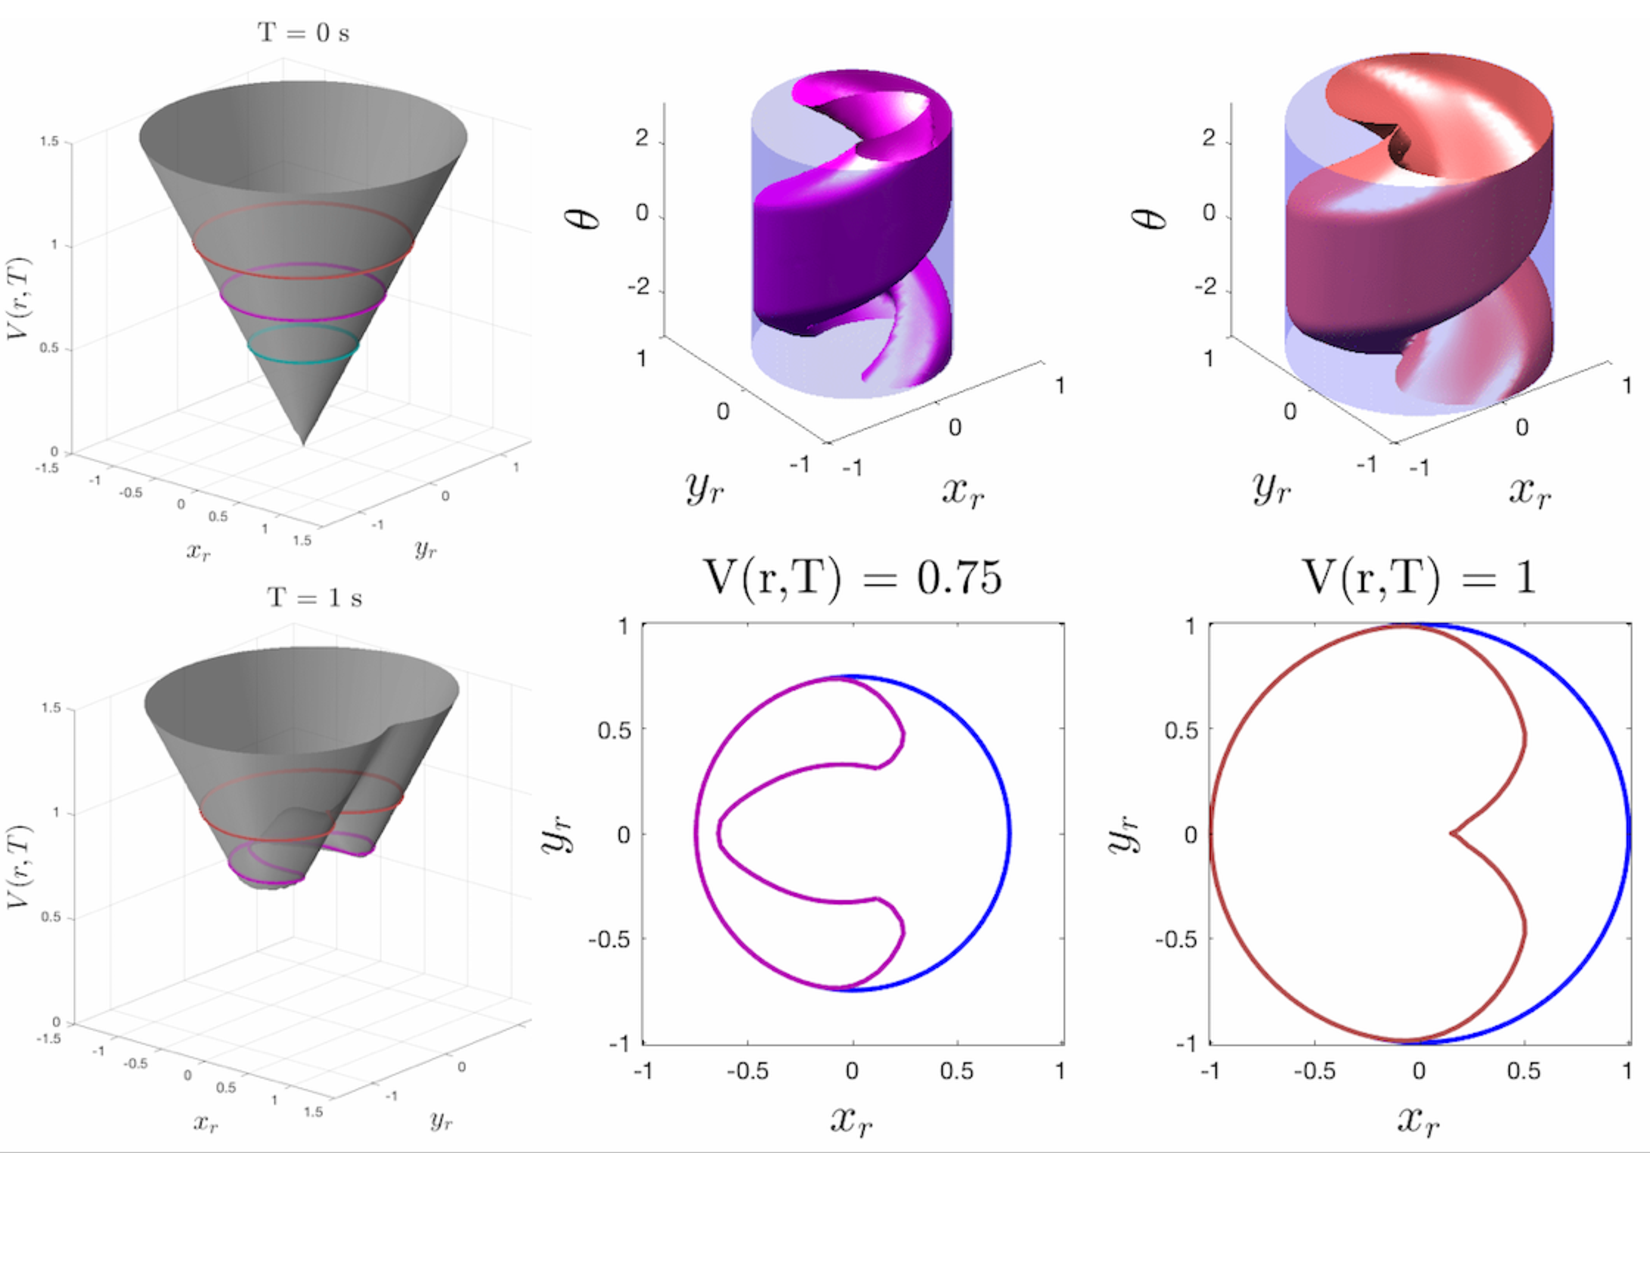
\includegraphics[width=0.5\textwidth]{fig/test}%quad4D_example}
%	\caption{Example of the precomputation for a 3D dubins car tracking a 2D kinematic planning model. The left side shows the cost function $\errfunc(\rstate)$ at $\theta = 0$, and its corresponding converged value function $\valfunc(\rstate)$. Level sets of the functions are shown in full 3D on the top right and at the 2D slice of $\theta=0$ on the bottom right.  If the initial relative state is contained within the inner set, the system is guaranteed to remain within the outer set. To find the $\TEB$ we select the smallest viable level set (in this case, 0.75 m).}
%	\label{fig:quad4D_example}
%	\vspace{-.2in}
%\end{figure} 


We want to find the farthest distance (and thus highest cost) that this game will ever reach when both players are acting optimally. Therefore we want to find a mapping between the initial relative state of the system and the maximum possible cost achieved over the time horizon. This mapping is through the value function, defined as
 \begin{align}
 \label{eq:valfunc}
 	V(\rstate,&\,\thor)= \sup_{\gamma_{\pstate} \in \Gamma_\pstate(t), \gamma_{\dstb} \in \Gamma_\dstb(t)} \inf_{\tctrl(\cdot) \in \tcfset(t)} \big\{\notag\\
 &\;\;\;\max_{\tvar\in [0, \thor]} \errfunc\Big(\rtraj(\tvar; \rstate, 0, \tctrl(\cdot), \gamma_\pstate[\tctrl](\cdot), \gamma_\dstb[\tctrl](\cdot))\Big)\big\}.
 	\end{align}

The tracking error function can be computed using dynamic programming by solving a corresponding HJ PDE over some time horizon \cite{Mitchell05, Fisac15}. If the control authority of the tracking system is powerful enough to always eventually reach the planning system, this value function will converge, $\valfunc_\infty(\rstate) := \lim_{\thor\rightarrow\infty} \valfunc(\rstate, \thor)$. In the next section we will prove that the sub-level sets of this value function will map initial relative states to the guaranteed furthest possible tracking error over all time, as seen in Fig. \ref{fig:quad10D_example}.
 
In the context of the online framework, $\valfunc_\infty(\rstate)$ is the tracking error bound function. The gradient of the value function, $\deriv_\infty(\rstate)$, inform the safety controller function (as described in Section \ref{sec:online}). When the framework is executed on a computer, these two functions are saved as look-up tables over a grid representing the relative state space.
 
\subsection{Invariance of Converged Value Function}
 \begin{prop}
   \label{prop:main}
   Suppose that the value function converges, and define $\valfunc_\infty(\rstate) := \lim_{\thor\rightarrow\infty}\valfunc(\rstate, T)$. Then $\forall \tvar_1, \tvar_2$ with $\tvar_2 \ge \tvar_1$, $\valfunc_\infty(\rstate) \ge \valfunc_\infty\Big(\rtraj^*(\tvar_2; \rstate, \tvar_1)\Big)$, where

   \begin{align}
   &\rtraj^*(\tvar; \rstate, 0) := \rtraj(\tvar; \rstate, 0, \tctrl^*(\cdot), \pctrl^*(\cdot), \dstb^*(\cdot))), \\
   %%%
   &\tctrl^*(\cdot) = \arg \inf_{\tctrl(\cdot)\in\tcfset(t)}\big\{\notag\\
   & \qquad \max_{\tvar \in [0, \thor]} \errfunc(\rtraj(\tvar; \rstate, 0, \tctrl(\cdot), \pctrl^*(\cdot), \dstb^*(\cdot))) \big\},\\
    %%%
   & \pctrl^*(\cdot) := \gamma_\pstate^*[\tctrl](\cdot) = \arg \sup_{\gamma_{\pstate} \in \Gamma_\pstate(t)} \inf_{\tctrl(\cdot) \in \tcfset(t)} \big\{\notag \\
   & \qquad \max_{t \in [0, \thor]} \errfunc(\rtraj(\tvar; \rstate, 0, \tctrl(\cdot), \gamma_\pstate[\tctrl](\cdot), \dstb^*(\cdot))) \big\}, \\
    %%%
   & \dstb^*(\cdot) = \arg \sup_{\gamma_{\dstb} \in \Gamma_\dstb(t)} \sup_{\gamma_{\pstate} \in \Gamma_\pstate(t)} \inf_{\tctrl(\cdot) \in \tcfset(t)} \big\{\notag\\
   & \qquad \max_{\tvar \in [0, \thor]} \errfunc(\rtraj(\tvar; \rstate, 0, \tctrl(\cdot), \gamma_\pstate[\tctrl](\cdot), \gamma_\dstb[\tctrl](\cdot))) \big\}.
   \end{align}
 \end{prop}

Proposition \ref{prop:main} proves that every level set of $\valfunc_\infty(\rstate)$ is invariant under the following conditions:
\begin{enumerate}
  \item The tracking system applies the optimal control which tries to track the planning system.
  \item The planning system applies (at worst) the optimal control that tries to escape from the tracking system. \label{ln:plan}
  \item The tracking system experiences (at worst) the optimal disturbance that tries to prevent successful tracking. \label{ln:dist}
\end{enumerate}
In practice, the worst case in conditions \ref{ln:plan} and \ref{ln:dist} may not occur; the result of this is only advantageous to the tracking system and will make it easier to stay within its current level set of $\valfunc_\infty(\rstate)$, or to move to a smaller invariant level set of $\valfunc_\infty(\rstate)$. The smallest invariant level set corresponding to the value $\underline\valfunc := \min_{\rstate} \valfunc_\infty(\rstate)$ can be interpreted as the smallest possible tracking error of the system. The tracking error bound is given by\footnote{In practice, since $\valfunc_\infty$ is obtained numerically, we set $\TEB = \{\rstate: \valfunc_\infty(\rstate) \le \underline\valfunc + \epsilon\}$ for some suitably small $\epsilon>0$} the set $\TEB = \{\rstate: \valfunc_\infty(\rstate) \le \underline\valfunc\}$. This tracking error bound in the planner's frame of reference is given by:
\begin{equation} \label{eq:TEBp}
\TEB_\pstate(\tstate) = \{\pstate: \valfunc_\infty(\tstate-\ptmat\pstate) \le \underline\valfunc\}.
\end{equation}
This is the tracking error bound that will be used in the online framework as shown in Fig. \ref{fig:fw_online}. Within this bound the tracking system may use any controller; on the border of this bound the tracking system must use the optimal controller. 

%We now prove Proposition \ref{prop:main}.
%\begin{proof}
%Without loss of generality, assume $\tvar_1=0$. By definition, we have
%\begin{equation}
%\begin{aligned}
%\valfunc_\infty(\rstate) & = \lim_{\thor\rightarrow\infty}\max_{\tvar \in [0, \thor]} \errfunc(\rtraj^*(\tvar; \rstate, 0))\\
%\end{aligned}
%\end{equation}
%By time-invariance, for some $\tvar_2 > 0$,
%\begin{equation}
%\label{eq:valfunc_ineq}
%  \begin{aligned}
%\valfunc_\infty(\rstate) &= \lim_{\thor\rightarrow\infty}\max_{\tvar \in [-\tvar_2, \thor]} \errfunc(\rtraj^*(\tvar; \rstate, -\tvar_2)) \\
%&\ge \lim_{\thor\rightarrow\infty}\max_{\tvar \in [0, \thor]} \errfunc(\rtraj^*(\tvar; \rstate, -\tvar_2)) 
%  \end{aligned}
%\end{equation}  
%\noindent where the sub-interval $[-\tvar_2, 0)$ has been removed in the last line. Next, by time invariance again, we  have
%\begin{equation}
%\begin{aligned}
%\rtraj^*(\tvar; \rstate, -\tau) &= \rtraj^*(\tvar; \rtraj^*(0; \rstate, -\tvar_2), 0) \\
%&= \rtraj^*(\tvar; \rtraj^*(\tvar_2; \rstate, 0), 0)
%\end{aligned}
%\end{equation}
%Now, \eqref{eq:valfunc_ineq} implies
%\begin{equation}
%\begin{aligned}
%\valfunc_\infty(\rstate) &\ge \lim_{\thor\rightarrow\infty}\max_{\tvar \in [0, \thor]} \errfunc(\rtraj^*(\tvar; \rtraj^*(\tvar_2; \rstate, 0), 0)) \\
%&= \valfunc_\infty(\rtraj^*(\tvar_2; \rstate, 0))
%\end{aligned}
%\end{equation} 
%\end{proof} 
 \begin{rem} 
   The proof of Proposition \ref{prop:main} can be found in \cite{ChenThesis}. The results are very similar to well-known results in differential game theory with a slightly different cost function \cite{Akametalu2014}, and has been utilized in the context of using the subzero level set of $\valfunc_\infty$ as a backward reachable set \cite{Mitchell05}. In our work we do not assign special meaning to any particular level set, and instead consider all level sets at the same time. This effectively allows us to perform solve many simultaneous reachability problems in a single computation, thereby removing the need to check whether resulting invariant sets are empty, as was done in \cite{Bansal2017}.
 \end{rem}